\chapter{Was ist die RoboNight?}

\section{RoboNight für Schüler}
Einen spielerischer Zugang zur Technik ist unerlässlich, wenn es darum geht, Schüler für einen technischen Studiengang zu begeistern und Interesse für technische Berufe zu fördern. Der spielerische Prozess sollte dabei so gestaltet sein, dass die Schüler dabei schnell selbst kreativ Ideen umsetzen und gestellte aufgaben meistern können. 

Als eine optimale Brücke zwischen Spielzeug und den Tätigkeiten eines Ingenieurs hat sich das Lego Mindstorms-System herauskristallisiert. Es erlaubt die Technische Problemstellungen auf ein Niveau zu skalieren, welches für Schüler geeignet ist, um sich selbst daran auszuprobieren, was die Neugier weckt. Mit dem Lego Mindstorms-System welches einen programmierbaren Stein und darauf abgestimmte Sensoren und Motoren beinhaltet können Roboter gebaut werden, die sowohl einfache als auch komplexe Aufgaben aus den Disziplinen der Mechanik, Konstruktion und Programmierung lösen können.

\begin{capfigure}[das Lego Mindstorms System]
	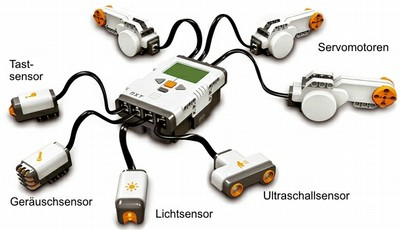
\includegraphics[width=10cm]{images/mindstorms.jpg}
 \end{capfigure}

Idealerweise werden die Roboter in kleinen Teams von 2-4 Personen konstruiert. Gemeinsames Bewältigen von Aufgaben fördert nicht nur das er- und miterleben des Lösungsprozesses und motiviert die Teilnehmer der Gruppe, sondern hilft auch schnell bei Schwierigkeiten durch unkomplizierte Hilfe der Teammitglieder untereinander.

Muss das Team auch noch gegen andere Teams antreten, werden die Teams durch den Wettbewerb angestachelt und bekommen durch die Lösungen der anderen Teams neue Ideen für die eigene Lösung.
  
Die Veranstaltung RoboNight bietet als Ergänzung zu den AGs in den Schulen zusätzliche Workshops an, bei denen sich die Schüler an vorgegebenen Aufgaben ausprobieren und ihre Lösungen vorführen dürfen. Außerdem bietet ein Vorentscheid die Möglichkeit, sich für den großen Abschluss der Workshops, der eigentlichen RoboNight zu qualifizieren. Die RoboNight ist ein Wettbewerb, bei dem die teilnehmenden Teams Roboter konstruieren müssen, die gestellte aufgaben lösen. Eine Jury vergibt Punkte für Kreativität und Innovation und entscheidet bei Streitfällen.

\section{RoboNight für Studenten}
Neben den sichtbaren Teil der RoboNight mit den Workshops und Wettbewerben besteht die RoboNight aus einem Verborgenen Teil. Dieser Betrifft die Organisation der RoboNight wie z.B. die gestellten Aufgaben, die Hilfestellungen bei den Workshops, deren Durchführung etc. Hier wird ein doppelter Lernansatz verfolgt, indem die RoboNight als Nichttechnisches Wahlpflichtfach ausgeschrieben wird. Studenten wird die Möglichkeit geben, sich an der Organisation und Durchführung zu beteiligen und gleichzeitig das eigene Studium durch den Erhalt von Creditpoints voranzutreiben. Eine win win.Situation.
  
\subsection{Inhalt des Wahlpflichtfachs RoboNight}
Das Wahlpflichtfach umfasst folgende Tätigkeiten:
 
\begin{itemize}
	\item Bearbeitung der Aufgabenstellungen (für Workshops und Wettbewerb)
	\item Realisierung und Erstellung von Musterlösungen
	\item Durchführung und Betreuung von 3 Workshops
	\item Betreuung beim Wettbewerb
	\item Nachbearbeitung und Dokumentation der Erfahrungen
\end{itemize}

\subsection{Lernziele}
 Aus den o.g. Tätigkeiten lassen sich klare Lernziele für die Studenten ableiten. Bevor die Studenten die Aufgabenstellungen ausarbeiten können, müssen sie sich sowohl mit der grafischen als auch mit der herkömmlichen Programmierung vertraut machen. Dies gilt insbesondere für den Workflow, um später kompetente Hilfestellung leisten zu können. Von der mechanischen Seite Betrachtet, müssen die Studenten die Möglichkeiten, die ein Standardkasten der Mindstorms Serie bietet einschätzen können, um den Schwierigkeitsgrad der Aufgaben richtig zu dimensionieren. Die Schwierigkeiten liegen hierbei nicht auf der Suche nach den Lösungen. Das Wie ist entscheidend und die Fähigkeit sich auf den Wissenstand der Schüler zu versetzen und auf deren Bedürfnisse einzugehen. Dies Betrifft auch die Durchführung des RoboNight Workshops. Es sollen Softskills erworben werden, die einen flexiblen Umgang mit etwaigen Problemen ermöglichen.  


\subsection{Modulbeschreibung}
Das Fach RoboNight ist ein nichttechnisches Wahlpflichtfach, welches mit 3 ECTS-Punkte bewertet ist. Die Präsenzzeit des Moduls umfasst bei 15 Semesterwochen 30 Stunden. Für die Vor- und Nachbearbeitung stehen 60 Stunden zur Verfügung.

Der Leistungsnachweis erfolgt zum über die Anwesenheit und Arbeit bei 3 der 4 Workshops und dem Vorentscheid. Ein anderer Teil besteht in der Erstellung der Aufgaben und deren Dokumentation. \autocite{Quelle: http://moduldb.htw-saarland.de/cgi-bin/moduldb-c?bkeys=yst&ckeys=kdvrw&lang=de}
    
    